\input{../common}
\everymath{\displaystyle}
\begin{document}
  %<*content>
  \lesson{algebra}{11}{ Statistique   à deux variables (TS2)}

\subsection{Généralités }
\subsection*{Statistique à une variable - Rappels :}
Soit X un caractère étudié dans une population d’effectif N, prenant les valeurs $ x_{i} $ $( 1\leq i \leq p)$.\\
A chaque modalité $ x_{i} $ on associe son effectif $ n_{i} $.\\
$n_{1} + n_{2} + \cdots+ n_{p}  =  N$


\begin{definition}

\begin{itemize}
\item L’ensemble des couples $(x_i, n_i)$ est appelé série statistique simple ou série statistique à une variable.
\item La fréquence de la modalité $x_i$ est le réel noté $f_i$ tel que : $f_i = \dfrac{n_i}{N}$
\item La moyenne de la série statistique $(x_i,n_i)$ est le réel noté  $ \overline{x} $ ou       $ \overline{X} $ tel que : $$ \overline{x} = \dfrac{n_{1}x_{1}+n_{2}x_{2}+\cdots +n_{p}x_{p}}{N}=\dfrac{1}{N}\sum_{i=1}^n n_{i}x_{i} $$
\item La variance de la série statistique  $(x_i,n_i)$  est le réel noté  $V(x)$ ou $V(X)$ tel que :
$$V(x)= \dfrac{n_{1}\paren{x_{1}-\overline{x}}^{2}+n_{2}\paren{x_{2}-\overline{x}}^{2}+\cdots +n_{p}\paren{x_{p}-\overline{x}}^{2}}{N}=\dfrac{1}{N}\displaystyle\sum_{i=1}^n n_{i}\paren{x_{i}-\overline{x}}^{2}$$
\end{itemize}
L’écart-type est la racine carrée de la variance. On le note  $ \sigma _{x} $ ou $ \sigma_X $. $\qquad \sigma_x=\sqrt{V(x)} $
\end{definition}

\begin{property}

 $$ Vx) = \dfrac{n_{1}x_{1}^{2}+n_{2}x_{2}^{2}+\cdots +n_{p}x_{p}^{2}}{N}-\overline{x}^{2}=\frac{1}{N}\sum_{i=1}^p n_{i}x_{i}^{2} -\overline{x}^{2}$$
\end{property}

\begin{remark}
 Lorsque la série est groupée en classes ; les centres de classes représentent $ x_i $.
 \end{remark}
Dans chacun des exercices  ci-dessous, calculer la moyenne, la variance et l’écart type de la série statistique donnée.


\medskip
 \begin{exercice}
 On considère la série de notes d’élèves de TS1, à un devoir de maths.

\medskip 


  $ \begin{array}{|c|c|c|c|c|c|c|c|c|}
\hline
\text{Notes}  x_{i}  & 7&  14&13&15&  10 &8 &9& 11 \\
 \hline
\end{array}$

\end{exercice} 


 \begin{exercice}
 Une enquête portant sur le nombre x de frères et sœurs d’élèves d’une seconde S a donné les résultats suivants :
 

  $ \begin{array}{|c|c|c|c|c|}
\hline
\text{ Nbre de frères et soeurs}  x_{i}  & 1&2&3&4 \\
 \hline
\text{ Effectifs } n_{i} &6&11&13&12\\
 \hline
\end{array}$
\end{exercice}


 \begin{exercice}

L'étude de la taille des élèves d’une classe a donné les résultats ci- dessous :


   $\begin{array}{|c|c|c|c|c|}
\hline
\text{ Classes} & [150 ;154[& [154  ;158[ &[158 ;162[&[162; 164[\\
 \hline
\text{ Effectifs} & 10 & 14 & 19 & 7 \\
 \hline
\end{array}$
\end{exercice}
\subsection{Série statistiques à deux variables}
On considère dans une population d’effectif $ N $, deux caractères $X$ et $Y$ prenant respectivement les valeurs  $x_1, x_2,\cdots,x_p$ et $  y_1, y_2, \cdots, y_q$. A tout couple $(x_i,y_j)$ , $i\in \{1,2,\cdots,p\}$ et $j\in \{1,2, \cdots,q\}$, on associe le nombre $n_{ij}$ d’individus pour lesquels $X$ prend la valeur $x_i$ et $Y $ la valeur $y_j$.

\begin{definition}

\begin{itemize}
\item L’ensemble des triplets $(x_i,y_j, n_{ij})$ est appelé série statistique double ou à deux variables associée au couple de caractère $(X,Y)$.\\
$n_{ij}$ est l’effectif du couple $(x_i,y_j)$
\item La fréquence du couple $(x_i , y_j)$ est : $ \dfrac{n_{ij}}{N} $;\; on la note $ f_{ij} $.\qquad  \fbox{$ f_{ij}= \frac{n_{ij}}{N}$}
\end{itemize}


\end{definition}


\begin{example} 
Le tableau ci-dessous donne les notes X de maths et Y de sciences physiques obtenues par 10 candidats au Bac S1 :

\medskip


   $\begin{array}{|c|c|c|c|c|c|c|c|c|c|c|}
\hline
  x_i & 7& 8 & 12&  11 &  14  &10 & 15 & 10  &12 & 10\\
 \hline
  y_i  & 8 & 11 & 9 & 13& 13 &9 &17 &12 &11&9 \\
 \hline
\end{array}$

L’effectif du couple $(11 ;13)$ est $1$ . La fréquence du couple $(11 ;13)$ est $\dfrac{1}{10} =0,1$.\\
L’effectif du couple $(10;9)$ est $2$.\\
Les modalités du caractère X sont :
 7-8-10-11-12-14-15.\\
Les modalités du caractère Y sont :
8-9-11-12-13-17.

\end{example}
\medskip

\begin{example}
Une enquête sur 100 familles portant sur le nombre d’enfants X par famille et le nombre de pièces d’habitation Y par famille a donné les résultats suivants.


\[

\begin{array}{|l|c|c|c|c|c|c|c|}
\hline
Y \backslash X & 0 & 1 & 2 & 3 & 4 & 5 & n_{\bullet j} \\
\hline
1 & 8 & 2 & 1 & 0 & 0 & 0 &  \\
\hline
2 & 3 & 11 & 10 & 5 & 1 & 0 &  \\
\hline
3 & 1 & 3 & 16 & 13 & 4 & 1 &  \\
\hline
4 & 0 & 1 & 3 & 5 & 8 & 4 &  \\
\hline
n_{i \bullet} &  &  &  &  &  &  &  \\
\hline
\end{array}
\]


L’effectif du couple $(1 ;2)$ est $11$ : il y a $11$ familles ayant $1$ enfant et $2$ pièces d’habitation.\\
La fréquence du couple $(2 ;2)$  est $ \dfrac{10}{100}=0,1$ : $10\%$ des familles ont $2$ enfants et deux pièces d’habitation.

\end{example}

\subsection*{Séries marginales}

A l’aide du tableau de l’exemple 9 précédent, on peut reconstituer la série statistique de chacun des caractères $X$ et $Y$ associés à cette série statistique double et de calculer leur moyenne, variance et écart -type.\\
L’effectif d’une valeur $x_i$ prise par $X$ est obtenu en additionnant les nombres $n_{i j}$ situés sur la même colonne que $x_i$ et on porte ce résultat en marge du tableau. L’effectif de $x_i$ est noté $ n_{i \bullet} $\\
$ n_{i \bullet} =\displaystyle\sum _{j=1}^{q}n_{i j} $\\
La série simple $(x_i, n_{i \bullet} )$ est appelée série (ou distribution) marginale de $X$.\\
De même, l’effectif d’une valeur $y_j$ prise par $Y$ est obtenu en additionnant les nombres $ n_{i j}$ situés sur la même ligne que $y_j$, et on porte ce résultat en marge du tableau. L’effectif de $x_j$ est noté $n_{\bullet j}$\\
$ n_{ \bullet   j} =\displaystyle\sum _{i=1}^{p}n_{i j} $\\
La série simple $(y_j,n_{\bullet j} )$ est appelée série ou distribution marginale de $Y$.

\begin{definition}

Les nombres $ n_{i \bullet} $ et  $ n_{\bullet j} $  sont les effectifs marginaux respectifs  de $x_i$ et $y_j$.\\
Les fréquences marginales sont les nombres $f_{i \bullet} $ et $f_{ \bullet   j}$ définis par: \[ f_{i \bullet}=\frac{n_{i \bullet}}{N} \quad \text{et} \quad  f_{ \bullet  j}=\frac{n_{ \bullet  j}}{N}  \]


\end{definition}

\subsection*{Séries ou distributions conditionnelles}
A partir de la distribution statistique double, on peut fixer la valeur d’un caractère et étudier la distribution qui en résulte pour l’autre caractère. On obtient ainsi deux types de séries conditionnelles: la distribution conditionnelle de $Y$ sachant que $X= x_i$ notée $(Y /X_i)$ et la distribution conditionnelle de $X$ sachant que $Y= y_j$ notée $(X/Y_j)$\\
La distribution conditionnelle $(Y /X_i)$  est la distribution de  $ n_{i \bullet} $ valeurs de $Y$ lorsque $X$ a pris une valeur fixée $x_i$ , c’est la série $(y_j,n_{i j})$ d’effectif total $n_{i \bullet}$.\\
On obtient les fréquences conditionnelles  de cette distribution:     $ \quad f(y_j/X_i)=\dfrac{n_{i j}}{n_{i \bullet}} $\\
Dans le tableau de l’exemple 9 précédent, on peut s’intéresser qu’aux familles à deux enfants et déterminer le nombre de pièces d’habitation qu’elles ont. Il y en a $30$.\\On obtient ainsi la série conditionnelle de $Y$ sachant que $X=2$\\
On peut extraire cette série du tableau :


   $\begin{array}{|c|c|c|c|c|}
\hline
  y_i & 1& 2 & 3&  4   \\
 \hline
\text{Effectifs} & 1 & 10 & 16 & 3 \\
 \hline
\end{array}$

Parmi les familles à deux enfants la fréquence de
celles qui ont 4 pièces d’habitation est $ \dfrac{3}{30}=0.1 $\\
C’est la fréquence conditionnelle de 4 sachant que
$X=2$. On note $f(4/2)=\dfrac{3}{30}=0.1$.\\
On en déduit que $10\%$ des familles à deux enfants
ont 4 pièces d’habitation.\\
La moyenne conditionnelle de $Y$ sachant $X=2$ est  égale à :                                  $ \overline{Y/2}=\dfrac{1\times 2 +2\times 10 +3\times 16+ 4\times 3}{30} =2,7$\\

\textbf{Interprétation}\\
Les familles à deux enfants ont
en moyenne 3 pièces d’habitation.

\begin{remark}
Les distributions conditionnelles $(Y / X _i )$ sont
présentées sous forme de fréquences
conditionnelles. En multipliant par 100 ces
fréquences on obtient la distribution conditionnelle
$(Y / X _i )$ en pourcentage, ce qui est conforme aux
habitudes de la vie.
\end{remark}
\begin{exercice}
Donner en pourcentage la distribution conditionnelle de la série double de l’exemple 9. Pour cela compléter le tableau suivant.


$
\begin{array}{|l|c|c|c|c|c|c|}
\hline
Y \backslash X\; \text{fixé} & 0 & 1 & 2 & 3 & 4 & 5  \\
\hline
1 &  &  &  &  &  &    \\
\hline
2 &  &  & &  &  &   \\
\hline
3 &  &  &  &  &  &    \\
\hline
4 &  &  &  &  &  &    \\
\hline
\text{Total} &  &  &  &  &  &    \\
\hline
\end{array}
$


\end{exercice}
\subsection{Nuage de points-Point moyen}
Soit $(x_i ,y_j ,n_{ij} )$ une série double associée au couple
de caractères $(X,Y)$.  Dans un plan muni d’un repère
orthogonal, on représente les points de
coordonnées $(x_i ,y_j )$. Et on indique à côté de chaque
point, l’effectif $n_{ij}$ s’il est différent de $1$ ou bien on
représente chacun de ces points par une tâche dont
l’étendue est proportionnelle à l’effectif\\
L’ensemble de ces points est appelé \textbf{nuage} de
la série double.

\begin{example}
\textbf{Nuage de la série double étudiée à
l’exemple 8}

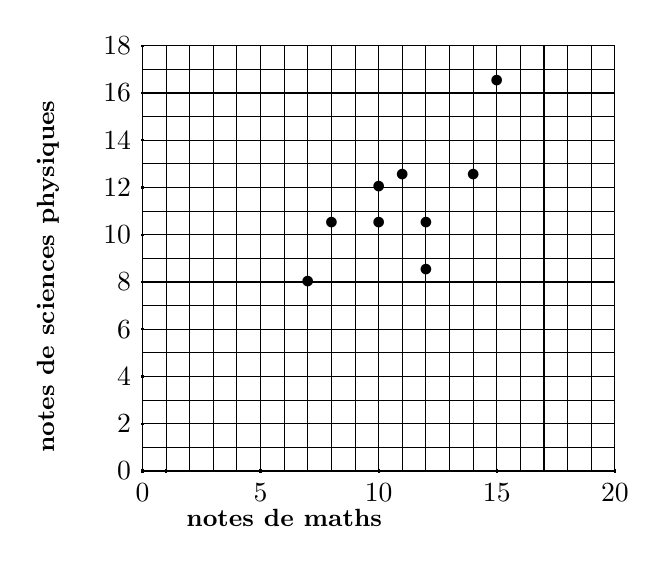
\begin{tikzpicture}[scale= 0.3 ]
\draw  (0,0) grid  (20,18) ;
\foreach\x in {0,,,,,5,,,,,10,,,,,15,,,,,,20}
{
\draw[thick] (\x,0.1) -- (\x,-0.1) node[below] {\x};
}
\foreach\y in {0,2,4,6,8,10,12,14,16,18}
{
\draw[thick] (0.05,\y) -- (-0.05,\y) node[left] {\y};
}
\node  at (-4,8)
             {\rotatebox{90}{\bf{ \small notes de sciences physiques}}};
  \node  at (6,-2)
             {\rotatebox{0}{\bf{\small notes de maths}}};
   \node at(7,8) {$ \bullet $};
   \node at(8,10.5) {$ \bullet $};
   \node at(10,10.5) {$ \bullet $};
   \node at(10,12) {$ \bullet $};
   \node at(11,12.5) {$ \bullet $};
    \node at(12,8.5) {$ \bullet $};
     \node at(12,10.5) {$ \bullet $};
      \node at(14,12.5) {$ \bullet $};
       \node at(15,16.5) {$ \bullet $};
\end{tikzpicture}



\textbf{ Nuage de la série double étudiée à
l’exemple 9}

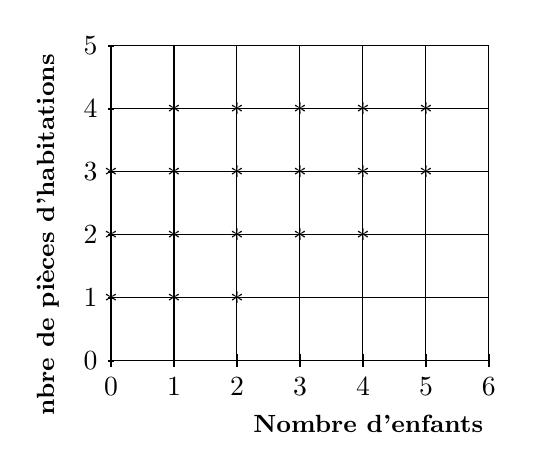
\begin{tikzpicture}[scale= 0.8 ]
\draw  (0,0) grid  (6,5) ;
\foreach\x in {0,1,2,3,4,5,6}
{
\draw[thick] (\x,0.1) -- (\x,-0.1) node[below] {\x};
}
\foreach\y in {0,1,2,3,4,5}
{
\draw[thick] (0.05,\y) -- (-0.05,\y) node[left] {\y};
}
\node  at (-1,2)
             {\rotatebox{90}{\bf{\small nbre de pièces d'habitations}}};
  \node  at (4,-1)
             {\rotatebox{0}{\bf{ \small Nombre d'enfants}}};
   \node at(0,1) {$ \ast $};
   \node at(0,2) {$ \ast $};
   \node at(0,3) {$ \ast $};
     \node at(1,1) {$ \ast $};
   \node at(1,2) {$ \ast $};
   \node at(1,3) {$ \ast $};
   \node at(1,4) {$ \ast $};
   \node at(2,1) {$ \ast $};
   \node at(2,2) {$ \ast $};
   \node at(2,3) {$ \ast $};
   \node at(2,4) {$ \ast $};
   \node at(3,2) {$ \ast $};
   \node at(3,3) {$ \ast $};
   \node at(3,4) {$ \ast $};
    \node at(4,2) {$ \ast $};
   \node at(4,3) {$ \ast $};
   \node at(4,4) {$ \ast $};
     \node at(5,3) {$ \ast $};
   \node at(5,4) {$ \ast $};
   \end{tikzpicture}
\end{example}

\medskip

Le barycentre $ G$ des points $M_{ij} (x_i ,y_j )$  affectés des
coefficients $ n _{ij}$ a pour coordonnées $( \overline{X} , \overline{Y} )$.\\
$ \overline{X} $ est la moyenne de la série marginale $X$ et  $ \overline{Y} $
celle de la série marginale $Y$.\\
Le point  $ G(  \overline{X} , \overline{Y}  )$ est appelé \textbf{point moyen}.

\subsection{Ajustement linéaire}
\subsection*{Notion d'ajustement}
Un nuage représentant une série statistique double
peut avoir différents aspects.\\
Ajuster un nuage par une courbe c’est trouver la
courbe la « plus proche » des points du nuage.
Cette courbe est appelée courbe d’ajustement ou
de régression ou d’estimation. Si cette courbe est
une droite, on parle de régression linéaire.
\subsection*{Ajustement linéaire par la méthode des moindres carrées}
On considère le nuage de $n$ points $M_{i} (x_i ,y_i )$.\\
$1\leq i \leq n$  d’effectifs tous égaux à $1$, représentant une
série statistique double $(X,Y)$.
\begin{center}
\begin{tikzpicture}[>=stealth', scale=1]
\clip (-1,-1) rectangle (7,5);
\draw[->,very thick] (-1,0) -- (7,0);
\draw[->,very thick] (0,-1) -- (0,5);

%\draw[thick,blue!50!black] plot[domain=-7:0.24,samples=100] (\x,{(2*\x+1)/(4*\x-1)}) node[above left] {$\mathscr{C}$};
\draw[very thick,red] plot[domain=-1:7,samples=100] (\x,{0.5*\x+1}) node[above left] {$ (D)$};
\draw[blue , dashed, very thick] (1,2.5) -- (1,3) node [above]{ $ M_{1}  $};
\draw[ dashed,very thick] (1,2.5) -- (1,1.3) node { $ P_{1}  $};
\draw[ dashed,very thick] (1,3) -- (4,3) node[above] { $ Q_{1}  $};
\draw[blue , dashed,very thick] (2 ,2) -- (2,4) node [above]{ $ M_{2}  $};
\draw[ dashed,very thick] (2,4) -- (2 ,1.7) node { $ P_{2}  $};
\draw[ dashed,thick] (2,4) -- (6,4) node[above] { $ Q_{2}  $};
\draw[blue , dashed,very thick] (3 ,2.5) -- (3,1) node [above right]{ $ M_{3}  $};
\draw[ dashed,very thick] (3,1) -- (0 ,1) node[above left] { $ Q_{3}  $};
\draw[ dashed,very thick] (3,2.5) -- (3,2.5) node[above] { $ P_{3}  $};
\draw[blue , dashed,very thick] (5.5 ,3.7) -- (5.5,2) node [above right]{ $ M_{4}  $};
\draw[ dashed,very thick](5.5 ,3.7)  -- (5.5 ,3.7) node[above  left] { $ P_{4}  $};
\draw[blue , dashed,very thick](5.5,2)-- (2 ,2)  node [above left]{ $ Q_{4}  $};
\end{tikzpicture}
\end{center}
Essayons d’approcher ce nuage par une droite
$ (D) $.\\
Supposons que les points ne sont pas tous situés
sur une droite parallèle à l’axe des ordonnées c’est
à dire $ X $ n’est pas une constante. On désigne $P_i$ le
projeté de $ M_i$ sur la droite $ (D) $ parallèlement à
l’axe des ordonnées.\\
Supposons que les points ne sont pas tous situés
sur l’axe des ordonnées, c’est à dire $Y$ n’est pas
une constante. On désigne $Q_i$ le projeté de $M_i$ sur
la droite $ (D) $ parallèlement à l’axe des abscisses.\\
La méthode des moindres carrées consiste à
chercher une droite $ (D) $ d’équation $ y= a x +b$ qui
rend minimale la somme des  $ M_{i}P_{i}^{2} $  ou une droite $ x'=a'y+b' $ qui
rend minimale la somme des  $ M_{i}Q_{i}^{2} $:\\
 $ M_{i}P_{i}^{2}=\paren{y_{i}-ax_{i}-b}^{2} $ \\
 $ M_{i}Q_{i}^{2}=\paren{x_{i}-a'y_{i}-b'}^{2} $ \\
 Dans le premier cas $(D)$ est appelée droite de
régression de $Y$ en $X$. On la note $D _{Y/X }$.\\
Dans le deuxième cas $(D)$ est appelée droite de
régression de $X$ en $Y$. On la note $ D _{X/Y}$ .

\begin{definition}

Soit $ \overline{X} $ et $ \overline{Y} $ les moyenne des séries
marginales associées à la série double $(X,Y)$
d’effectif $N$. On appelle \textit{covariance } de $(X,Y)$ le
réel noté cov$(X,Y)$ ou   $ \sigma _{XY} $ défini par : 

\[\text{cov}(X,Y)=\frac{n_{11}x_{1}y_{1}+n_{12}x_{1}y_{2}+\cdots+n_{pq}x_{p}y_{q}}{ N}  -\overline{X}\overline{Y}\]
\end{definition}

\begin{remark}
cov$ (X,X)=V(X)  \quad  \text{et} \quad cov (Y,Y)=V(Y) $
\end{remark}

\begin{theorem}
\begin{itemize}
\item La droite de régression de Y en X passe par le
point moyen et a pour équation : $\; y-\overline{y}=a(x-\overline{x})\;$ où  $\; a=\dfrac{\text{cov}(X,Y)}{V(X)} $.
\item La droite de régression de X en Y passe par le
point moyen et a pour équation : $\; x-\overline{x}=a'(y-\overline{y})\; $ où  $\; a'=\dfrac{\text{cov}(X,Y)}{V(Y)} $.
\end{itemize}

\end{theorem}


\begin{remark}
 Ces équations permettent de trouver
par extrapolation à partir d’une valeur de x fixée,
la valeur de y estimée et inversement.
\end{remark}

\begin{exercice}
Déterminer les droites de régression de Y en X et de
X en Y des séries doubles étudiées aux exemples  8 et 9).
\end{exercice}
\subsection*{Coefficient de corrélation linéaire}
Lorsque les points du nuage sont groupés suivant
une direction rectiligne, on a une dépendance
statistique linéaire entre les caractères X et Y. On
dit qu’il y a corrélation linéaire entre X et Y.

\begin{definition}


On appelle coefficient de corrélation linéaire d’une série statistique double $(X ;Y)$ le réel $ r $ défini
par :  $$ r=\dfrac{\text{cov}(X,Y)}{\sqrt{V(X)V(Y)}}   \quad \text{ou} \quad  r=\dfrac{\text{cov}(X,Y)}{\sigma_{X}\sigma_{Y}}  $$

 \end{definition}
 
 \begin{property}
 
 \begin{itemize}
 \item[$ \bullet $] $ r^{2}=aa' $ où  $a $ et $ a’ $  sont les coefficients directeurs
respectifs des droites de régression de Y en X et de
X en Y.
\item[$ \bullet $]  $ -1\leq r \leq 1 $
\end{itemize}
 \end{property}

\begin{remark}
\begin{itemize}
 \item Si  $ a< 0 \;$  et $\; a'< 0\; $  alors $\; r=-\sqrt{aa'} $
\item Si  $ a> 0\; $  et $\; a'> 0\;$  alors $ \; r=\sqrt{aa'} $
\end{itemize}
\end{remark}
\subsection*{Appréciation de la corrélation linéaire }
Le réel $ \abs{r} $ permet d’apprécier la corrélation
linéaire entre les variables X et Y.\\
  $ \bullet\; $  Si  $ 0,87 \leq |r| \leq1  $  alors la corrélation linéaire
entre les deux variables est forte.\\
 $ \bullet\; $ Si  $ | r | < 0,87 $ la corrélation est faible.
 \begin{remark}
  Si la corrélation est faible, un
ajustement linéaire n’est pas justifié.
\end{remark}




  %</content>
\end{document}